\documentclass[lualatex,handout]{beamer}
\setbeamertemplate{footline}[frame number]
\usepackage{luatexja}
\usepackage{amsmath,amssymb}

%\usetheme{Berlin}
\usecolortheme{rose}

\usepackage{tikz}
\usepackage{pgfplots}
\pgfplotsset{compat=1.18}

%\usepackage[haranoaji]{luatexja-preset}
\usepackage[deluxe,ipaex]{luatexja-preset}
\renewcommand{\kanjifamilydefault}{\gtdefault}
%\setmainjfont{HaranoAjiGothic-Regular}

\usepackage{unicode-math}
%\setmathfont{Fira Math}
\setmathfont{STIX Two Math}
\setmathrm{STIX Two Math}[StylisticSet=8]

%\usefonttheme{professionalfonts}

\usepackage{luacolor}

\newcommand{\emm}[1]{\textcolor{red}{#1}}
\newcommand{\expt}[1]{\mathbb{E}\left[#1\right]}
\newcommand{\var}[1]{\mathbb{V}\left[#1\right]}
\newcommand{\cov}[1]{\mathrm{Cov}\left[#1\right]}


\usepackage{xspace}
\newcommand\bm[1]{{\mathbf{#1}}}
\newcommand\dx{{\,\mathrm{d}x}}

\theoremstyle{definition}

\title{確率・統計基礎: 大数の法則と集中不等式}
\author{森 立平}
\date{}



\begin{document}
\begin{frame}[plain]
\maketitle
\end{frame}

\begin{frame}{集中不等式}

確率変数$X_1,X_2,\dotsc,X_N$が\emm{独立}で\emm{同一の分布}に従うとき、
独立同分布(independently and identically distributed (i.i.d.))であるという。

\vspace{1em}
このスライドでは$X_1,\dotsc,X_N$は i.i.d.で確率変数$X$と同分布であると仮定する。

\vspace{1em}
\emm{$N$個のi.i.d.確率変数の平均$\frac{\sum_{k=1}^NX_k}{N}$が期待値$\expt{X}$周辺に集中}するというのが大数の法則や集中不等式が示すことである。
\end{frame}

\begin{frame}{二項分布}
\begin{align*}
\Pr(X = k) &= \binom{n}{k} p^k(1-p)^{n-k},\quad \emm{n=30},\, p=0.3.
\end{align*}
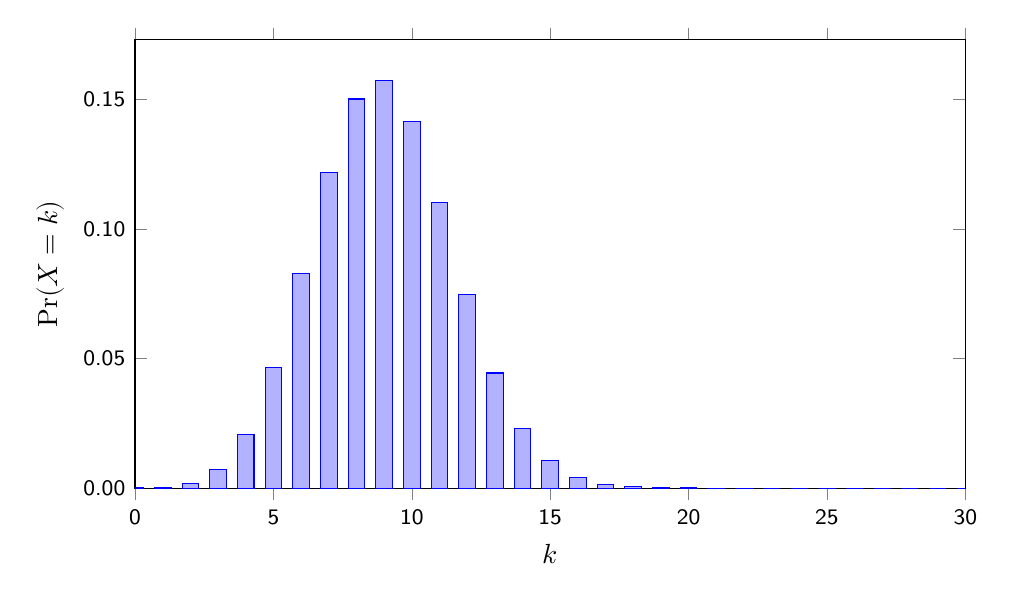
\begin{tikzpicture}[%
declare function={binom(\k,\n,\p)=\n!/(\k!*(\n-\k)!)*\p^\k*(1-\p)^(\n-\k);}]
\pgfmathsetmacro{\binomN}{30}
\begin{axis}[
    width=\textwidth, height=\axisdefaultheight,
    ylabel={$\Pr(X=k)$},
    xlabel={$k$},
    xmin=0, xmax=\binomN,
    ymin=0,
    scaled ticks = false,
    tick label style={/pgf/number format/assume math mode=true, font=\footnotesize\sffamily},
    yticklabel style={/pgf/number format/.cd, fixed, fixed zerofill, precision=2},
        domain=0:\binomN,samples at={0,1,...,\binomN},
    mark options={scale=0.75, blue},
    ybar, bar width = 6pt
        ]
%\addplot[ycomb] {binom(x,\binomN,0.3)};
\addplot {binom(x,\binomN,0.3)};
\end{axis}
\end{tikzpicture}
\end{frame}

\begin{frame}{二項分布}
\begin{align*}
\Pr(X = k) &= \binom{n}{k} p^k(1-p)^{n-k},\quad \emm{n=60},\, p=0.3.
\end{align*}
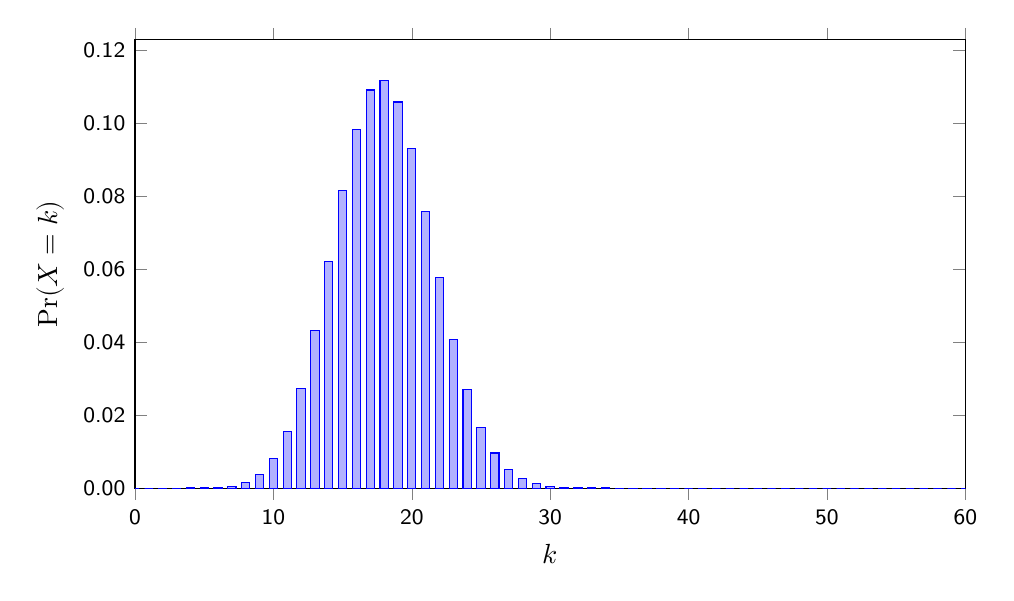
\begin{tikzpicture}[%
declare function={binom(\k,\n,\p)=\n!/(\k!*(\n-\k)!)*\p^\k*(1-\p)^(\n-\k);}]
\pgfmathsetmacro{\binomN}{60}
\begin{axis}[
    width=\textwidth, height=\axisdefaultheight,
    ylabel={$\Pr(X=k)$},
    xlabel={$k$},
    xmin=0, xmax=\binomN,
    ymin=0,
    scaled ticks = false,
    tick label style={/pgf/number format/assume math mode=true, font=\footnotesize\sffamily},
    yticklabel style={/pgf/number format/.cd, fixed, fixed zerofill, precision=2},
        domain=0:\binomN,samples at={0,1,...,\binomN},
    mark options={scale=0.75, blue},
    ybar, bar width = 3pt
        ]
%\addplot[ycomb] {binom(x,\binomN,0.3)};
\addplot {binom(x,\binomN,0.3)};
\end{axis}
\end{tikzpicture}
\end{frame}

\begin{frame}{二項分布}
\begin{align*}
\Pr(X = k) &= \binom{n}{k} p^k(1-p)^{n-k},\quad \emm{n=120},\, p=0.3.
\end{align*}
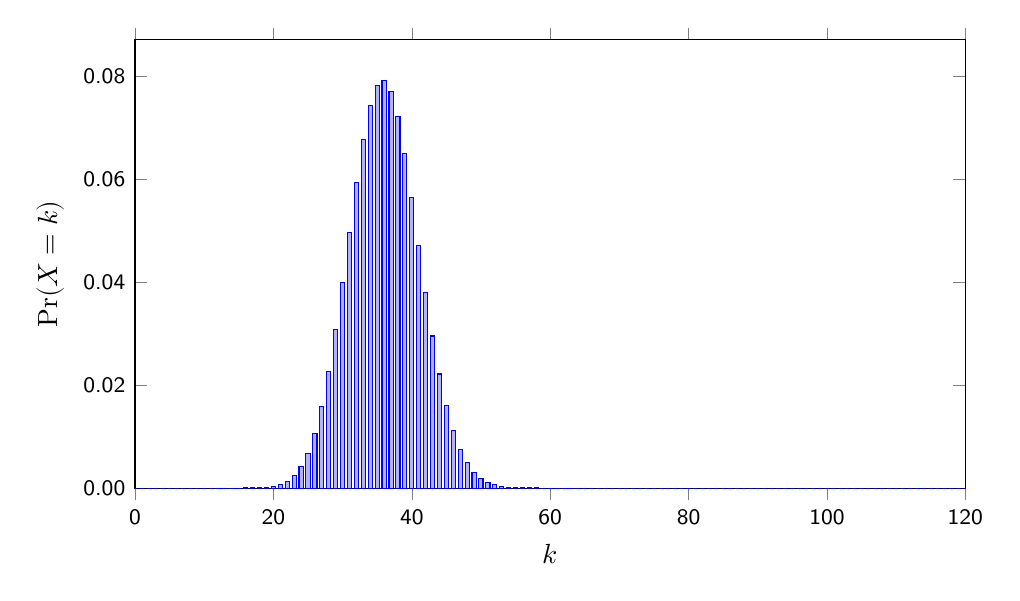
\begin{tikzpicture}[%
declare function={binom(\k,\n,\p)=\n!/(\k!*(\n-\k)!)*\p^\k*(1-\p)^(\n-\k);}]
\pgfmathsetmacro{\binomN}{120}
\begin{axis}[
    width=\textwidth, height=\axisdefaultheight,
    ylabel={$\Pr(X=k)$},
    xlabel={$k$},
    xmin=0, xmax=\binomN,
    ymin=0,
    scaled ticks = false,
    tick label style={/pgf/number format/assume math mode=true, font=\footnotesize\sffamily},
    yticklabel style={/pgf/number format/.cd, fixed, fixed zerofill, precision=2},
        domain=0:\binomN,samples at={0,1,...,\binomN},
    mark options={scale=0.75, blue},
    ybar, bar width = 1.5pt
        ]
%\addplot[ycomb] {binom(x,\binomN,0.3)};
\addplot {binom(x,\binomN,0.3)};
\end{axis}
\end{tikzpicture}
\end{frame}

\begin{frame}{二項分布}
\begin{align*}
\Pr(X = k) &= \binom{n}{k} p^k(1-p)^{n-k},\quad \emm{n=240},\, p=0.3.
\end{align*}
\begin{tikzpicture}[%
declare function={binom(\k,\n,\p)=\n!/(\k!*(\n-\k)!)*\p^\k*(1-\p)^(\n-\k);}]
\pgfmathsetmacro{\binomN}{240}
\pgfmathsetmacro{\p}{0.3}
\begin{axis}[
    width=\textwidth, height=\axisdefaultheight,
    ylabel={$\Pr(X=k)$},
    xlabel={$k$},
    xmin=0, xmax=\binomN,
    ymin=0,
    scaled ticks = false,
    tick label style={/pgf/number format/assume math mode=true, font=\footnotesize\sffamily},
    yticklabel style={/pgf/number format/.cd, fixed, fixed zerofill, precision=2},
        domain=0:\binomN,samples at={0,1,...,\binomN},
    mark options={scale=0.75, blue},
    ybar, bar width = .75pt
        ]
%\addplot[ycomb] {binom(x,\binomN,0.3)};
%\addplot {binom(x,\binomN,0.3)};
\addplot[domain=0:\binomN, color=blue, samples={\binomN+1}, thick] gnuplot { exp(lgamma(\binomN+1) - lgamma(x+1) - lgamma(\binomN-x+1) + x*log(\p) + (\binomN-x)*log(1-\p)) with impulses};
\end{axis}
\end{tikzpicture}
\end{frame}

\begin{frame}{二項分布}
\begin{align*}
\Pr(X = k) &= \binom{n}{k} p^k(1-p)^{n-k},\quad \emm{n=480},\, p=0.3.
\end{align*}
\begin{tikzpicture}[%
declare function={binom(\k,\n,\p)=\n!/(\k!*(\n-\k)!)*\p^\k*(1-\p)^(\n-\k);}]
\pgfmathsetmacro{\binomN}{480}
\pgfmathsetmacro{\p}{0.3}
\begin{axis}[
    width=\textwidth, height=\axisdefaultheight,
    ylabel={$\Pr(X=k)$},
    xlabel={$k$},
    xmin=0, xmax=\binomN,
    ymin=0,
    scaled ticks = false,
    tick label style={/pgf/number format/assume math mode=true, font=\footnotesize\sffamily},
    yticklabel style={/pgf/number format/.cd, fixed, fixed zerofill, precision=2},
        domain=0:\binomN,samples at={0,1,...,\binomN},
    mark options={scale=0.75, blue},
    ybar, bar width = .375pt
        ]
%\addplot[ycomb] {binom(x,\binomN,0.3)};
%\addplot {binom(x,\binomN,0.3)};
\addplot[domain=0:\binomN, color=blue, samples={\binomN+1}, thick] gnuplot { exp(lgamma(\binomN+1) - lgamma(x+1) - lgamma(\binomN-x+1) + x*log(\p) + (\binomN-x)*log(1-\p)) with impulses};
%\addplot[domain=0:\binomN, thick] gnuplot {x};
\end{axis}
\end{tikzpicture}
\end{frame}

\begin{frame}{二項分布}
\begin{align*}
\Pr(X = k) &= \binom{n}{k} p^k(1-p)^{n-k},\quad \emm{n=1000},\, p=0.3.
\end{align*}
\begin{tikzpicture}[%
declare function={binom(\k,\n,\p)=\n!/(\k!*(\n-\k)!)*\p^\k*(1-\p)^(\n-\k);}]
\pgfmathsetmacro{\binomN}{1000}
\pgfmathsetmacro{\p}{0.3}
\begin{axis}[
    width=\textwidth, height=\axisdefaultheight,
    ylabel={$\Pr(X=k)$},
    xlabel={$k$},
    xmin=0, xmax=\binomN,
    ymin=0,
    scaled ticks = false,
    tick label style={/pgf/number format/assume math mode=true, font=\footnotesize\sffamily},
    yticklabel style={/pgf/number format/.cd, fixed, fixed zerofill, precision=2},
        domain=0:\binomN,samples at={0,1,...,\binomN},
    mark options={scale=0.75, blue},
    ybar, bar width = .375pt
        ]
%\addplot[ycomb] {binom(x,\binomN,0.3)};
%\addplot {binom(x,\binomN,0.3)};
\addplot[domain=0:\binomN, color=blue, samples={\binomN+1}, thick] gnuplot { exp(lgamma(\binomN+1) - lgamma(x+1) - lgamma(\binomN-x+1) + x*log(\p) + (\binomN-x)*log(1-\p)) with impulses};
%\addplot[domain=0:\binomN, thick] gnuplot {x};
\end{axis}
\end{tikzpicture}
\end{frame}

\begin{frame}{二項分布}
\begin{align*}
\Pr(X = k) &= \binom{n}{k} p^k(1-p)^{n-k},\quad \emm{n=10000},\, p=0.3.
\end{align*}
\begin{tikzpicture}[%
declare function={binom(\k,\n,\p)=\n!/(\k!*(\n-\k)!)*\p^\k*(1-\p)^(\n-\k);}]
\pgfmathsetmacro{\binomN}{10000}
\pgfmathsetmacro{\p}{0.3}
\begin{axis}[
    width=\textwidth, height=\axisdefaultheight,
    ylabel={$\Pr(X=k)$},
    xlabel={$k$},
    xmin=0, xmax=\binomN,
    ymin=0,
    scaled ticks = false,
    tick label style={/pgf/number format/assume math mode=true, font=\footnotesize\sffamily},
    yticklabel style={/pgf/number format/.cd, fixed, fixed zerofill, precision=3},
        domain=0:\binomN,samples at={0,1,...,\binomN},
    mark options={scale=0.75, blue},
    ybar, bar width = .375pt
        ]
%\addplot[ycomb] {binom(x,\binomN,0.3)};
%\addplot {binom(x,\binomN,0.3)};
\addplot[domain=0:\binomN, color=blue, samples={\binomN+1}, thick] gnuplot { exp(lgamma(\binomN+1) - lgamma(x+1) - lgamma(\binomN-x+1) + x*log(\p) + (\binomN-x)*log(1-\p)) with impulses};
%\addplot[domain=0:\binomN, thick] gnuplot {x};
\end{axis}
\end{tikzpicture}
\end{frame}

\if0
\begin{frame}{二項分布}
\begin{align*}
\Pr(X = k) &= \binom{n}{k} p^k(1-p)^{n-k},\quad \emm{n=20000},\, p=0.3.
\end{align*}
\begin{tikzpicture}[%
declare function={binom(\k,\n,\p)=\n!/(\k!*(\n-\k)!)*\p^\k*(1-\p)^(\n-\k);}]
\pgfmathsetmacro{\binomN}{20000}
\pgfmathsetmacro{\p}{0.3}
\begin{axis}[
    width=\textwidth, height=\axisdefaultheight,
    ylabel={$\Pr(X=k)$},
    xlabel={$k$},
    xmin=0, xmax=\binomN,
    ymin=0,
    scaled ticks = false,
    tick label style={/pgf/number format/assume math mode=true, font=\footnotesize\sffamily},
    yticklabel style={/pgf/number format/.cd, fixed, fixed zerofill, precision=2},
        domain=0:\binomN,samples at={0,1,...,\binomN},
    mark options={scale=0.75, blue},
    ybar, bar width = .375pt
        ]
%\addplot[ycomb] {binom(x,\binomN,0.3)};
%\addplot {binom(x,\binomN,0.3)};
\addplot[domain=0:\binomN, color=blue, samples={\binomN+1}, thick] gnuplot { exp(lgamma(\binomN+1) - lgamma(x+1) - lgamma(\binomN-x+1) + x*log(\p) + (\binomN-x)*log(1-\p)) with impulses};
%\addplot[domain=0:\binomN, thick] gnuplot {x};
\end{axis}
\end{tikzpicture}
\end{frame}
\fi


\begin{frame}{集中不等式}
\begin{theorem}[大数の弱法則]
確率変数$X$が\emm{分散を持つ}とする。
%$(X_k)_{k=1,\dotsc,}$が$X$と独立同分布とする。
このとき、任意の実数$\epsilon>0$について
\begin{align*}
\lim_{N\to\infty}\Pr\left(\left|\frac1N\sum_{k=1}^N X_k-\expt{X}\right|\ge \epsilon\right) &=0.
\end{align*}
\end{theorem}
\begin{proof}
チェビシェフの不等式より
\begin{align*}
\Pr\left(\left|\frac1N\sum_{k=1}^N X_k-\expt{X}\right|\ge \epsilon\right) &\le
\frac{\var{\frac1N\sum_{k=1}^NX_k}}{\epsilon^2} = \frac{\var{X}}{\epsilon^2\emm{N}}\stackrel{N\to\infty}{\longrightarrow} 0.
\end{align*}
\end{proof}
\end{frame}


\begin{frame}{チェルノフ上界}
\small
\begin{theorem}[チェルノフ上界]
%任意の実数$t>0$について
\begin{align*}
\Pr(X\ge a)&\le\frac{M_X(t)}{\mathrm{e}^{at}} = \mathrm{e}^{\emm{K_X(t) - at}} \qquad\forall t>0\\
\Pr(X\le a)&\le\frac{M_X(t)}{\mathrm{e}^{at}} = \mathrm{e}^{\emm{K_X(t) - at}} \qquad\forall t<0.
\end{align*}
\end{theorem}
\begin{proof}
任意の実数$t>0$について
\begin{align*}
\Pr(X\ge a)&=\Pr\bigl(\mathrm{e}^{tX}\ge\mathrm{e}^{ta}\bigr)\\
&\le\frac{\expt{\mathrm{e}^{tX}}}{\mathrm{e}^{ta}}\qquad\text{(Markovの不等式)}\\
&=\frac{M_X(t)}{\mathrm{e}^{ta}}.\qedhere
\end{align*}
任意の実数$t<0$について$\Pr(X\le a) = \Pr(\mathrm{e}^{tX}\ge \mathrm{e}^{ta})\le\frac{M_X(t)}{\mathrm{e}^{ta}}$.
\end{proof}
\end{frame}

\begin{frame}{チェルノフ上界の最適化}
任意の実数$t>0$について
\begin{align*}
\Pr(X\ge a)&\le\mathrm{e}^{K_X(t)-at}
\end{align*}
が成り立つので上界の最小化
\begin{align*}
\inf_{t>0} \mathrm{e}^{K_X(t)-at}
\end{align*}
を考えたい。$\log$とってから最小化すると
\begin{align*}
\inf_{t>0} \{K_X(t) - at\}
&=
-\sup_{t>0} \{at - K_X(t)\}
.
\end{align*}
\emm{キュムラント母関数}$K_X(t)$の\emm{ルジャンドル変換}
\end{frame}

\begin{frame}{キュムラント母関数の性質}
\begin{align*}
K_X(t) &= \log \expt{\mathrm{e}^{tX}}
\end{align*}
\begin{itemize}
\setlength{\itemsep}{2em}
\item $K_X(0) = 0$.
\item $t\in(-\epsilon,\epsilon)$でキュムラント母関数が存在すると仮定すると、$\left.\frac{\mathrm{d}K_X(t)}{\mathrm{d} t}\right|_{t=0} = \expt{X}$.
%\item $a \le \expt{X}$ のとき $K_X^*(a) = 0$.
\item ある$R>0$について$t\in(-R, R)$でキュムラント母関数が存在すると仮定すると、この範囲で$K_X(t)$は凸関数。
\end{itemize}
\end{frame}

\begin{frame}{キュムラント母関数の凸性}
\begin{align*}
K_X(t) &= \log \expt{\mathrm{e}^{tX}}
\end{align*}
$t\in(-R, R)$でキュムラント母関数が存在すると仮定すると、この範囲で\emm{微分と期待値を交換できる}。
% \sum_{k=0}^n |(x^k)/k! t^k| <= exp(|tx|) <= exp(tx) + exp(-tx)
% E[\sum_{k=0}^n |(x^k)/k! t^k|] <= M_X(t) + M_X(-t)
%
% \sum_{k=0}^n |f^{(k)}(s)/k! (tx-s)^k| <= exp(|tx-s|+s) <= exp(tx) + exp(2s-tx) ???
\begin{align*}
\frac{\mathrm{d} K_X(t)}{\mathrm{d}t} &= \frac{\expt{X\mathrm{e}^{tX}}}{\expt{\mathrm{e}^{tX}}}\\
\frac{\mathrm{d}^2 K_X(t)}{\mathrm{d}t^2} &= \frac{\expt{X^2\mathrm{e}^{tX}}\expt{\mathrm{e}^{tX}}-\expt{X\mathrm{e}^{tX}}^2}{\expt{\mathrm{e}^{tX}}^2}\\
&= \frac{\expt{X^2\mathrm{e}^{tX}}}{\expt{\mathrm{e}^{tX}}}-\left(\frac{\expt{X\mathrm{e}^{tX}}^2}{\expt{\mathrm{e}^{tX}}}\right)^2\\
&= \frac{\expt{\left(X-\frac{\expt{X\mathrm{e}^{tX}}}{\expt{\mathrm{e}^{tX}}}\right)^2\mathrm{e}^{tX}}}{\expt{\mathrm{e}^{tX}}}\ge 0
\end{align*}
\end{frame}

\begin{frame}{ルジャンドル変換}
\begin{definition}
$J\subseteq\mathbb{R}$を区間とし、関数$f\colon J\to\mathbb{R}$を\emm{凸関数}とする。
$f$の\emm{ルジャンドル変換}$f^*\colon J^*\to\mathbb{R}$を以下で定義する。
\begin{align*}
f^*(a) &= \emm{\sup_{t\in J}\{at - f(t)\}}\\
J^*&=\{a\in\mathbb{R}\mid f^*(a)<\infty\}
\end{align*}
\end{definition}

\vspace{1em}
$f$は凸なので、$at-f(t)$は$t$の関数として凹(上に凸)となる。
このとき、
\begin{itemize}
\setlength{\itemsep}{1em}
\item $f'(t^*) = a$ を満たす$t^*\in J$が存在するとき、$f^*(a) = at^* - f(t^*)$である。
$f'$が単調非減少であることから、$t^*$は$a$について単調非減少である。
%\item $\lim_{t\to\inf(J)} f'(t) > a$ のときや$\lim_{t\to\sup(J)} f'(t) < a$のとき、$f^*(a)=\infty$である。
\end{itemize}
\end{frame}

\begin{frame}{凸関数と接線}
\centering
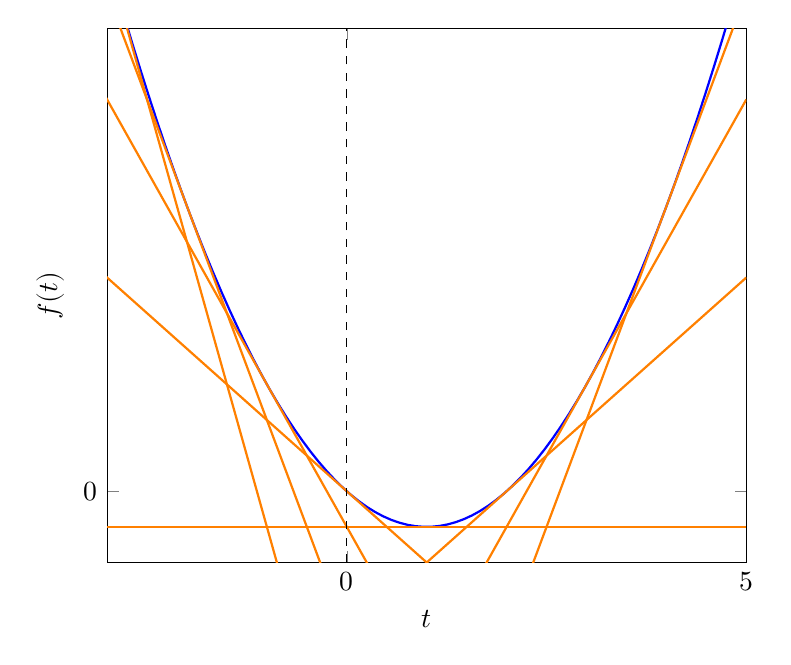
\begin{tikzpicture}
\begin{axis}[
    width=0.8\textwidth,
    xlabel=$t$,
    ylabel=$f(t)$,
    xmin=-3, xmax=5,
    ymin=-2, ymax=13,
    xtick={0,5},
    ytick={0},
    legend pos = south east
]
    \addplot[domain=-5:5, samples=100, color=blue, thick] {-2*x+x^2};
    \addplot[domain=-5:5, samples=100, color=orange, thick] {-2*x};
    \addplot[domain=-5:5, samples=100, color=orange, thick] {-1};
    \addplot[domain=-5:5, samples=100, color=orange, thick] {2*(x-2) + 0};
    \addplot[domain=-5:5, samples=100, color=orange, thick] {4*(x-3) + 3};
    \addplot[domain=-5:5, samples=100, color=orange, thick] {6*(x-4) + 8};
    \addplot[domain=-5:5, samples=100, color=orange, thick] {(-4)*(x+1) + 3};
    \addplot[domain=-5:5, samples=100, color=orange, thick] {(-6)*(x+2) + 8};
    \addplot[domain=-5:5, samples=100, color=orange, thick] {(-8)*(x+3) + 15};
    %\addplot[domain=-5:5, samples=100, color=orange, thick] {3*(x-5/2) - 5 + 25/4};
    \draw[dashed, black] (axis cs:0, -2) -- (axis cs:0, 13);
    %\legend{$K_X(t)$, $\expt{X}t$}
\end{axis}
\end{tikzpicture}

\small
凸関数は接線の集合で表すことができる。
接線$at+b$は傾き$a$と切片$b$で表せる。
凸関数は同じ傾きを持つ接線が一つしかないので、\emm{傾きから切片が一意に定まる}。
この傾きから切片(の$-1$倍)への関数がルジャンドル変換$f^*$に他ならない。
\end{frame}

\begin{frame}{ルジャンドル変換}
%$f(0)=0$のときのルジャンドル変換$f^*(y) = \sup_{x\in\mathbb{R}} \{yx - f(x)\}$.
%$\sup$は$f'(x^*)=y$を満たす$x^*(y)$で達成される。
$f'(t^*) = a$より、$a=f'(0)$のとき、$t^*=0$である。特に$f(0)=0$のとき以下の図のようになる。

\vspace{1em}
\begin{center}
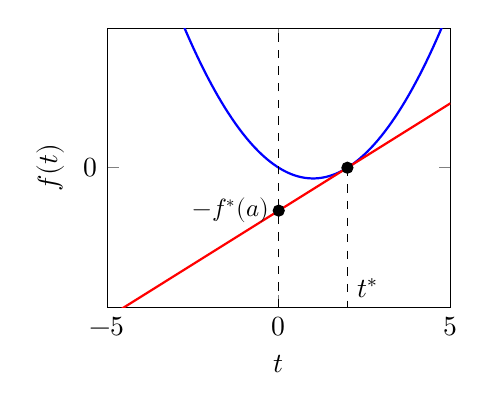
\begin{tikzpicture}
\begin{axis}[
    width=0.49\textwidth,
    xlabel=$t$,
    ylabel=$f(t)$,
    xmin=-5, xmax=5,
    ymin=-13, ymax=13,
    xtick={-5,0,5},
    ytick={0},
    legend pos = south east
]
    \addplot[domain=-5:5, samples=100, color=blue, thick] {-2*x+x^2};
    %\addplot[black, mark=*, only marks] coordinates {(0, 0)};
    \draw[dashed, black] (axis cs:0, -13) -- (axis cs:0, 13);
    %\addplot[domain=-5:5, samples=100, color=red, thick] {-2*x};
    \addplot[domain=-5:5, samples=100, color=red, thick] {2*(x-2) + 0};
    \addplot[black, mark=*, only marks] coordinates {(0, -4)};
    \node[left] at (axis cs:0, -4) {\small $-f^*(a)$};
    \addplot[black, mark=*, only marks] coordinates {(2, 0)};
    \draw[dashed, black] (axis cs:2, 0) -- (axis cs:2, -13);
    \node[above right] at (axis cs:2, -13) {$t^*$};
    %\node[left] at (axis cs:0, -4) {\tiny $y(x-x^*) + f(x^*)$};
    %\legend{$f(x)$, $a(x-x^*)+f(x^*)$}
\end{axis}
\end{tikzpicture}
\hfill
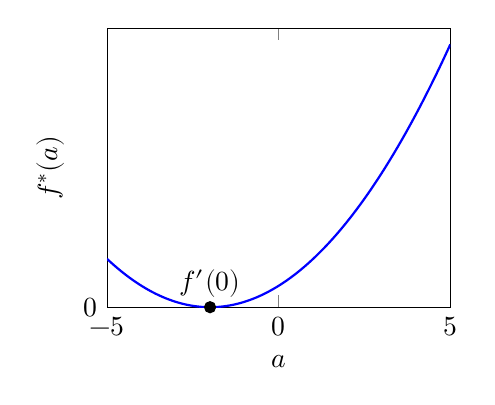
\begin{tikzpicture}
\begin{axis}[
    width=0.49\textwidth,
    xlabel=$a$,
    ylabel=$f^*(a)$,
    xmin=-5, xmax=5,
    ymin=0, ymax=13,
    xtick={-5,0,5},
    ytick={0},
    legend pos = south east
]
    \addplot[domain=-5:5, samples=100, color=blue, thick] {(x+2)^2/4};
    \addplot[black, mark=*, only marks] coordinates {(-2, 0)};
    \node[above] at (axis cs:-2, 0) {$f'(0)$};
    %\addplot[domain=-5:5, samples=100, color=red, thick] {-2*x};
    %\addplot[domain=-5:5, samples=100, color=red, thick] {2*(x-2) + 0};
    %\legend{$f(x)$, $a(x-x^*)+f(x^*)$}
\end{axis}
\end{tikzpicture}
\end{center}
$f^*(a)$ は$f$の傾きが$a$のところの接線$a(t-t^*) + f(t^*)$の$t=0$での値の$-1$倍。

$t^*$は$a=f'(0)$のとき0で$a>f'(0)$のとき、$t^*>0$、$a<f'(0)$のとき$t^*<0)$。
\end{frame}

\begin{frame}{チェルノフ上界の最適化}
\begin{lemma}
%任意の実数$t>0$について
\emm{レート関数}$I_X\colon\mathbb{R}\to\mathbb{R}_{\ge 0}$を
\begin{align*}
%I_+(a) &:= \sup_{t > 0}\left\{at - K_X(t)\right\}\\
%I_-(a) &:= \sup_{t < 0}\left\{at - K_X(t)\right\}
I_X(a) &:= \sup_{t \in\mathrm{dom}(K_X)}\left\{at - K_X(t)\right\}
\end{align*}
%とおくと、
と定義する。
このとき、
\begin{align*}
\sup_{t>0}\left\{at-K_X(t)\right\}&=\begin{cases}
I_X(a)&\text{if } a > \expt{X}\\
0&\text{otherwise.}
\end{cases}\\
\sup_{t<0}\left\{at-K_X(t)\right\}&=\begin{cases}
I_X(a)&\text{if } a < \expt{X}\\
0&\text{otherwise.}
\end{cases}
\end{align*}
%である。このとき任意の$a\in\mathbb{R}$について
%\begin{align*}
%\Pr(X\ge a)&\le \mathrm{e}^{-I(a)}\qquad\forall a>\expt{X}\\
%\Pr(X\le a)&\le \mathrm{e}^{-I(a)}\qquad\forall a<\expt{X}.
%\end{align*}
\end{lemma}
よってチェルノフ上界を最適化することで以下を得る。
\begin{align*}
\Pr\left(X\ge a\right) &\le \mathrm{e}^{-I_X(a)}\qquad\forall a>\expt{X}\\
\Pr\left(X\le a\right) &\le \mathrm{e}^{-I_X(a)}\qquad\forall a<\expt{X}.
\end{align*}
\end{frame}

\begin{frame}{集中不等式 by チェルノフ上界}
\small
\begin{theorem}[集中不等式]
\vspace{-1em}
\begin{align*}
%\Pr\left(\frac1N\sum_{k=1}^N X_k\ge a\right) &\le \mathrm{e}^{-K_X^*(a)N}.
% \mathrm{e}^{N(K_X(t) - at)}
\Pr\left(\frac1N\sum_{k=1}^N X_k\ge a\right) &\le \mathrm{e}^{-\emm{I_X(a)}N}\qquad\forall a>\expt{X}\\
\Pr\left(\frac1N\sum_{k=1}^N X_k\le a\right) &\le \mathrm{e}^{-\emm{I_X(a)}N}\qquad\forall a<\expt{X}.
\end{align*}
\end{theorem}
\begin{proof}
任意の$t>0$について
\begin{align*}
\Pr\left(\frac1N\sum_{k=1}^N X_k\ge a\right) &=
%\Pr\left(\exp\left(t\sum_{t=1}^N X_t\right)\ge \exp\left(t(\expt{X} + a)N\right)\right)\\
\Pr\left(\sum_{k=1}^N X_k\ge Na\right)\\
&\le\mathrm{e}^{K_{\sum_k X_k}(t) - Nat}\qquad\text{(チェルノフ上界)}\\
&=\mathrm{e}^{N(K_X(t) - at)}
\end{align*}
$t>0$を最適化することで補題を得る。
\end{proof}
\end{frame}



\begin{frame}{例: ベルヌーイ分布}
\begin{align*}
\Pr(X=0) &= 1-p,&\Pr(X=1)=p
\end{align*}
\begin{align*}
K_X(t) &= \log(p\mathrm{e}^t + (1-p))
\end{align*}
\begin{align*}
I_X(a) &= \sup_{t\in\mathbb{R}} \left\{ at - \log(p\mathrm{e}^t+(1-p))\right\}
\end{align*}
\begin{align*}
a - \frac{p\mathrm{e}^{t^*}}{p\mathrm{e}^{t^*}+1-p} = 0
\iff \mathrm{e}^{t^*} = \frac{a(1-p)}{p(1-a)}
\end{align*}
\begin{align*}
I_X(a) &= a\log\frac{a(1-p)}{p(1-a)} - \log\left(\frac{a(1-p)}{1-a} + (1-p)\right)\\
 %&= (a-1)\log\frac{1-p}{1-a} + a\log\frac{a}{p}
 &= \emm{a\log\frac{a}{p} + (1-a)\log\frac{1-a}{1-p}}
\end{align*}
\end{frame}

\begin{frame}{例: 正規分布}
%\small
\begin{align*}
p(x) &= \frac1{\sqrt{2\pi\sigma^2}} \mathrm{e}^{-\frac{(x-\mu)^2}{2\sigma^2}}\qquad\text{for}\quad x\in\mathbb{R}.
\end{align*}
\begin{align*}
M_X(t) &= \int_{-\infty}^\infty\frac1{\sqrt{2\pi\sigma^2}} \mathrm{e}^{-\frac{(x-\mu)^2}{2\sigma^2}} \mathrm{e}^{tx}\dx\\
 &= \int_{-\infty}^\infty\frac1{\sqrt{2\pi\sigma^2}} \mathrm{e}^{-\frac{(x-\mu -\sigma^2t)^2}{2\sigma^2}} \mathrm{e}^{\frac{(\mu+\sigma^2t)^2-\mu^2}{2\sigma^2}}\dx\\
&=\mathrm{e}^{\frac{(\mu+\sigma^2t)^2-\mu^2}{2\sigma^2}}
=\mathrm{e}^{\mu t + \frac{\sigma^2t^2}2}.
\end{align*}
\begin{align*}
K_X(t) &= \emm{\mu t + \frac{\sigma^2t^2}2}.\\
\end{align*}
\end{frame}

\begin{frame}{例: 正規分布}
\begin{align*}
K_X(t) &= \emm{\mu t + \frac{\sigma^2t^2}2}.\\
%\sup_{t>0} \left\{at - \left(\mu t + \frac{\sigma^2t^2}2\right)\right\} &= 
%\sup_{t>0} \left\{-\frac{\sigma^2}2 t\left(t-\frac{2(a-\mu)}{\sigma^2}\right) \right\}\\
% &= 
%\begin{cases}
%\emm{\frac{(a-\mu)^2}{2\sigma^2}}& a \ge \mu\\
%0&\text{otherwise.}
%\end{cases}
I_X(a)&=\sup_{t\in\mathbb{R}} \left\{at - \left(\mu t + \frac{\sigma^2t^2}2\right)\right\}\\
&= \sup_{t\in\mathbb{R}} \left\{-\frac{\sigma^2}2 t\left(t-\frac{2(a-\mu)}{\sigma^2}\right) \right\}\\
&=\emm{\frac{(a-\mu)^2}{2\sigma^2}}.
\end{align*}

\vspace{1em}
任意の$\epsilon>0$について
\begin{align*}
\Pr\left(\frac1N\sum_{k=1}^N X_k \ge \mu + \epsilon\right) &\le \mathrm{e}^{-\emm{\frac{\epsilon^2}{2\sigma^2}}N}\\
\Pr\left(\frac1N\sum_{k=1}^N X_k \le \mu - \epsilon\right) &\le \mathrm{e}^{-\emm{\frac{\epsilon^2}{2\sigma^2}}N}.
\end{align*}
\end{frame}

\begin{frame}{例: ポアソン分布}
\begin{align*}
\Pr(X=k) &= \frac{\lambda^k\mathrm{e}^{-\lambda}}{k!}\qquad\text{for}\quad k\in\mathbb{Z}_{\ge 0}.
\end{align*}
\begin{align*}
M_X(t) &= \sum_{k\ge 0}\frac{\lambda^k\mathrm{e}^{-\lambda}}{k!} \mathrm{e}^{tk}\\
&= \mathrm{e}^{\lambda\mathrm{e}^t - \lambda}\\
K_X(t) &= \emm{\lambda(\mathrm{e}^t-1)}
\end{align*}
\end{frame}

\begin{frame}{例: ポアソン分布}
\begin{align*}
K_X(t) &= \emm{\lambda(\mathrm{e}^t-1)}
\end{align*}
\begin{align*}
%\sup_{t>0}\left\{at - \lambda(\mathrm{e}^t-1)\right\}
I_X(a)&=\sup_{t\in\mathbb{R}}\left\{at - \lambda(\mathrm{e}^t-1)\right\}
\end{align*}
\begin{align*}
a-\lambda\mathrm{e}^{t^*} &= 0\iff t^* = \log \frac{a}{\lambda}
\end{align*}
\begin{align*}
%\sup_{t>0}\left\{at - \lambda(\mathrm{e}^t-1)\right\} &=
%\begin{cases}
%a\log\frac{a}{\lambda} -a + \lambda& a \ge \lambda\\
%0&\text{otherwise.}
%\end{cases}
I_X(a)&=\sup_{t\in\mathbb{R}}\left\{at - \lambda(\mathrm{e}^t-1)\right\}\\
 &= \emm{a\log\frac{a}{\lambda} -a + \lambda}.
\end{align*}

\vspace{.5em}
%任意の$\epsilon>0$について
%任意の$c > 1$について
\begin{align*}
%\Pr\left(\frac1N\sum_{k=1}^N X_k \ge \lambda+\epsilon\right) &\le \mathrm{e}^{-\emm{((\lambda+\epsilon) \log\frac{\lambda+\epsilon}{\lambda} - \epsilon)}N}.
\Pr\left(\frac1N\sum_{k=1}^N X_k \ge c\lambda\right) &\le \mathrm{e}^{-\emm{\lambda\left(c\log c -c + 1 \right)}N}\qquad\forall c > 1\\
\Pr\left(\frac1N\sum_{k=1}^N X_k \le c\lambda\right) &\le \mathrm{e}^{-\emm{\lambda\left(c\log c -c + 1 \right)}N}\qquad\forall c < 1\\
\end{align*}
\end{frame}

\begin{frame}{例: 指数分布}
%\small
\begin{align*}
p(x) &= \lambda\mathrm{e}^{-\lambda x}\qquad\text{for}\quad x\ge 0.
\end{align*}
\begin{align*}
M_X(t) &= \int_{0}^\infty \lambda\mathrm{e}^{-\lambda x} \mathrm{e}^{tx}\dx\\
&=\left[\frac{\lambda}{t-\lambda}\mathrm{e}^{(t-\lambda)x}\right]_0^{\infty}\\
&=\begin{cases}
\frac{\lambda}{\lambda-t}& t < \lambda\\
+\infty&\text{otherwise.}
\end{cases}
\end{align*}
\begin{align*}
K_X(t) &=
\begin{cases}
\emm{\log\frac{\lambda}{\lambda-t}}& t < \lambda\\
+\infty&\text{otherwise.}
\end{cases}
\end{align*}
\end{frame}

\begin{frame}{例: 指数分布}
\small
\begin{align*}
K_X(t) &=
\begin{cases}
\emm{\log\frac{\lambda}{\lambda-t}}& t < \lambda\\
+\infty&\text{otherwise.}
\end{cases}
\end{align*}
\begin{align*}
I_X(a) &= \sup_{t<\lambda} \left\{at - \log\frac{\lambda}{\lambda-t}\right\}
\end{align*}
\begin{align*}
a - \frac1{\lambda-t^*} &=0 \iff  t^* = \lambda-\frac1a
\end{align*}
\begin{align*}
I_X(a) &= \sup_{t<\lambda} \left\{at - \log\frac{\lambda}{\lambda-t}\right\}\\
&=
%\begin{cases}
\emm{a\lambda - 1 - \log(a\lambda)}
%& a > \frac1\lambda\\
%0 & \text{otherwise.}
%\end{cases}
\end{align*}

%\vspace{.5em}
%任意の$\epsilon>0$について
%任意の$c > 1$について
\begin{align*}
%\Pr\left(\frac1N\sum_{k=1}^N X_k \ge \lambda+\epsilon\right) &\le \mathrm{e}^{-\emm{((\lambda+\epsilon) \log\frac{\lambda+\epsilon}{\lambda} - \epsilon)}N}.
\Pr\left(\frac1N\sum_{k=1}^N X_k \ge \frac{c}{\lambda}\right) &\le \mathrm{e}^{-\emm{(c-1-\log c)}N} \qquad\forall c>1\\
\Pr\left(\frac1N\sum_{k=1}^N X_k \ge \frac{c}{\lambda}\right) &\ge \mathrm{e}^{-\emm{(c-1-\log c)}N} \qquad\forall c<1.
\end{align*}
\end{frame}


\begin{frame}{大偏差原理 Lv1}
レート関数$I_X(a)$は\emm{最適な指数}であり、これ以上改善することはできない。証明は難しいので紹介しない。
\begin{theorem}[クラメールの定理]
\begin{align*}
\lim_{N\to\infty}\frac1N \log \Pr\left(\frac1N\sum_{k=1}^N X_k \ge a\right) &= -I_X(a) \qquad\forall a>\expt{X}\\
\lim_{N\to\infty}\frac1N \log \Pr\left(\frac1N\sum_{k=1}^N X_k \le a\right) &= -I_X(a) \qquad\forall a<\expt{X}
\end{align*}
\end{theorem}
\end{frame}

\begin{frame}{サブガウシアン}
\small
キュムラント母関数やレート関数が綺麗に計算できればよいのだが、必ずしもそうとは限らない。

\vspace{1em}
\begin{definition}
$X$が代理分散$s^2>0$について\emm{サブガウシアン} $\stackrel{\mathrm{def}}{\iff}$ 任意の$t\in\mathbb{R}$について
\begin{align*}
%&\expt{\mathrm{e}^{t(X-\expt{X})}} \le \mathrm{e}^{\frac{s^2t^2}2}\\
%\iff&\expt{\mathrm{e}^{tX}} \le \mathrm{e}^{\expt{X}t+\frac{s^2t^2}2}\\
%\iff& 
K_X(t) &\le {\expt{X}t+\frac{s^2t^2}2}.
\end{align*}
\end{definition}

\vspace{1em}
キュムラント母関数を正規分布のキュムラント母関数で上から抑えることで、正規分布の場合と同じ形の不等式が得られる。

$X$が代理分散$s^2>0$について\emm{サブガウシアン}のとき、任意の$\epsilon>0$について
\begin{align*}
\Pr\left(\frac1N\sum_{k=1}^N X_k \ge \expt{X} + \epsilon\right) &\le \mathrm{e}^{-\emm{\frac{\epsilon^2}{2s^2}}N},&
\Pr\left(\frac1N\sum_{k=1}^N X_k \le \expt{X} - \epsilon\right) &\le \mathrm{e}^{-\emm{\frac{\epsilon^2}{2s^2}}N}.
\end{align*}
\end{frame}

\begin{frame}{有界な確率変数}
\small
\begin{lemma}[Hoeffiding's lemma]
確率変数$X$が
\begin{align*}
\Pr(X\in[a,b])&=1
\end{align*}
を満たすとする。このとき$X$は\emm{代理分散$\frac{(b-a)^2}4$}についてサブガウシアンである。
つまり、
\begin{align*}
K_X(t)=\log\expt{\mathrm{e}^{tX}} &\le \expt{X}t + \frac{(b-a)^2t^2}8.
\end{align*}
\end{lemma}
\begin{proof}
$X$が有界であることから、$K_X(t)$は任意の$t\in\mathbb{R}$について存在する。
テイラーの定理よりある$\theta\in(0,t)$が存在して、($t<0$のときは$\theta\in(t, 0)$)
\begin{align*}
K_X(t) &= \expt{X}t + K_X''(\theta)\frac{t^2}2
\end{align*}
ここで、$K_X''(\theta)$はある確率変数$Z\in[a,b]$の分散$\var{Z}$である。
\end{proof}
%\vspace{1em}
%実際$\Pr(X=a)=\Pr(X=b)=1/2$のとき、$\var{X} = \frac{(b-a)^2}4$である。
\end{frame}

\begin{frame}{Hoeffiding's lemma の証明}
\small
\begin{proof}[証明の続き]
\begin{align*}
K''_X(t) 
%&= \frac{\expt{X^2\mathrm{e}^{tX}}\expt{\mathrm{e}^{tX}}-\expt{X\mathrm{e}^{tX}}^2}{\expt{\mathrm{e}^{tX}}^2}\\
%&= \frac{\expt{X^2\mathrm{e}^{tX}}}{\expt{\mathrm{e}^{tX}}}-\left(\frac{\expt{X\mathrm{e}^{tX}}^2}{\expt{\mathrm{e}^{tX}}}\right)^2\\
&= {\expt{\left(X-\frac{\expt{X\mathrm{e}^{tX}}}{\expt{\mathrm{e}^{tX}}}\right)^2\mathrm{e}^{tX}}}/{\expt{\mathrm{e}^{tX}}}.
\end{align*}
具体的には
\begin{align*}
\Pr(Z\in A) &= \frac{\expt{\mathbb{I}_A(X)\mathrm{e}^{\theta X}}}{\expt{\mathrm{e}^{\theta X}}}
\end{align*}
という確率変数$Z$について、$K_X''(\theta) = \var{Z}$である。

例えば$X$の確率密度関数が$p(x)$のとき、$Z$の確率密度関数は$p(x)\frac{\mathrm{e}^{\theta x}}{\int_{-\infty}^\infty p(x)\mathrm{e}^{\theta x}\dx}$である。
$\Pr(Z\in[a,b])=1$である。
%任意の$x\in\mathbb{R}$について
\begin{align*}
\expt{(Z-x)^2} &= x^2 - 2\expt{Z}x + \expt{Z^2}\ge \var{Z}\qquad\forall x\in\mathbb{R}
%\var{Z} &= \expt{(Z-\expt{Z})^2}
\end{align*}
より、$x=\frac{a+b}2$を代入すると、
%\begin{align*}
$\var{Z} \le \expt{\left(Z-\frac{a+b}2\right)^2}\le \left(\frac{b-a}2\right)^2$.
%\end{align*}
\end{proof}
\end{frame}

\begin{frame}{Hoeffiding 不等式}
\begin{theorem}[Hoeffiding 不等式]
確率変数$X$が
\begin{align*}
\Pr(X\in[a,b])&=1
\end{align*}
を満たすとする。
任意の$\epsilon>0$について
\begin{align*}
\Pr\left(\frac1N\sum_{k=1}^N X_k \ge \expt{X} + \epsilon\right) &\le \mathrm{e}^{-\emm{\frac{2\epsilon^2}{(b-a)^2}}N}\\
\Pr\left(\frac1N\sum_{k=1}^N X_k \le \expt{X} - \epsilon\right) &\le \mathrm{e}^{-\emm{\frac{2\epsilon^2}{(b-a)^2}}N}.
\end{align*}
\end{theorem}
\end{frame}

\begin{frame}{おまけ: テイラーの定理}
\begin{theorem}[テイラーの定理]
実関数$f\colon\mathbb{R}\to\mathbb{R}$が$a\in\mathbb{R}$で$k\ge 1$回微分可能なとき、
ある関数$h_k\colon\mathbb{R}\to\mathbb{R}$で$\lim_{x\to a}h_k(x)=0$であるものが存在し、
\begin{align*}
f(x) &= \sum_{s=0}^k \frac{f^{(s)}(a)}{s!}(x-a)^s + h_k(x)(x-a)^k.
\end{align*}

また、$f\colon\mathbb{R}\to\mathbb{R}$が$[a, x]$上 で$k+1$回微分可能であるとすると、ある$c\in(a, x)$が存在し、
\begin{align*}
f(x) &= \sum_{s=0}^k \frac{f^{(s)}(a)}{s!}(x-a)^s + \frac{f^{(k+1)}(c)}{(k+1)!}(x-a)^{k+1}.
\end{align*}
\end{theorem}
\end{frame}

\begin{frame}{課題}
\begin{enumerate}
\setlength{\itemsep}{2em}
\item 表が出る確率が$1/2$のコインを$N$回投げて$0.6N$回以上表が出る確率を$\mathrm{e}^{-cN}$という形で上から抑えるときの最大の$c>0$をもとめよ。
\item 1から6の目を持つ偏りのないサイコロを$N$回投げて和の合計が$4N$以上になる確率$\mathrm{e}^{-cN}$という形で上から抑えるときの最大の$c>0$をもとめよ。
\end{enumerate}
\end{frame}

%\begin{frame}{大偏差原理 Lv2}
%\begin{theorem}[サノフの定理]
%\end{theorem}
%\end{frame}
\end{document}
